\documentclass[a4paper, 12pt]{scrartcl}

\usepackage{graphicx}
\usepackage[%
    font={small,sf},
    labelfont=bf,
    format=hang,    
    format=plain,
    margin=0pt,
    width=0.8\textwidth,
]{caption}
\usepackage[list=true]{subcaption}
\usepackage{placeins}

\begin{document}
CRA case - Model A

\begin{figure}[h!]
\centering
\subcaptionbox{NSGA}{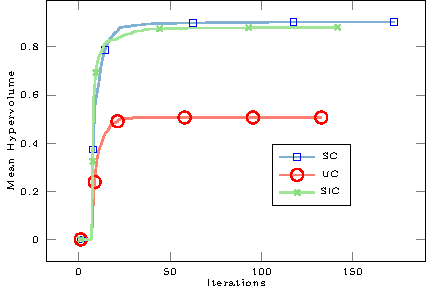
\includegraphics[width=0.3\textwidth]{CRA/NSGAII/charts/hypervolume/hv-mean-progression-a.pdf}}%
\hfill
\subcaptionbox{PESA2}{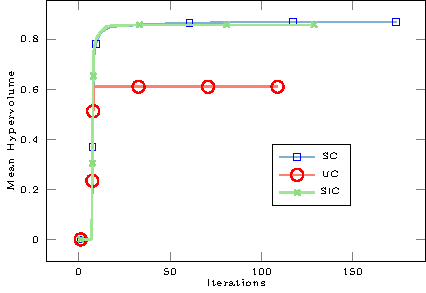
\includegraphics[width=0.3\textwidth]{CRA/PESA2/charts/hypervolume/hv-mean-progression-a.pdf}}%
\hfill
\subcaptionbox{SPEA2}{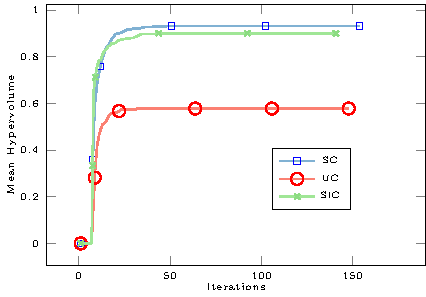
\includegraphics[width=0.3\textwidth]{CRA/SPEA2/charts/hypervolume/hv-mean-progression-a.pdf}}%
\hfill

\subcaptionbox{NSGA}{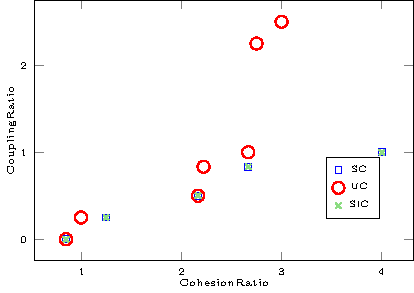
\includegraphics[width=0.3\textwidth]{CRA/NSGAII/charts/approximation_sets/approx-sets-A.pdf}}%
\hfill
\subcaptionbox{PESA2}{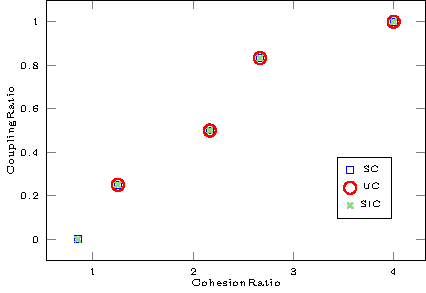
\includegraphics[width=0.3\textwidth]{CRA/PESA2/charts/approximation_sets/approx-sets-A.pdf}}%
\hfill
\subcaptionbox{SPEA2}{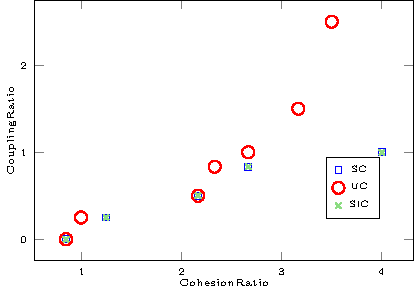
\includegraphics[width=0.3\textwidth]{CRA/SPEA2/charts/approximation_sets/approx-sets-A.pdf}}%
\hfill
\caption{Model A.}
\end{figure}

CRA case - Model B

\begin{figure}[h!]
\centering
\subcaptionbox{NSGA}{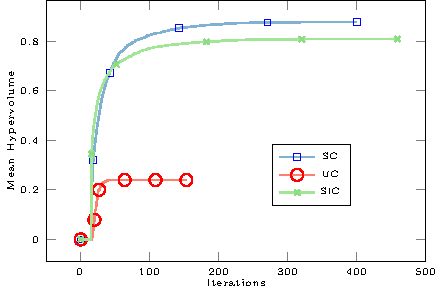
\includegraphics[width=0.3\textwidth]{CRA/NSGAII/charts/hypervolume/hv-mean-progression-b.pdf}}%
\hfill
\subcaptionbox{PESA2}{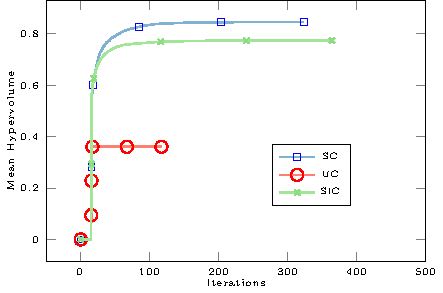
\includegraphics[width=0.3\textwidth]{CRA/PESA2/charts/hypervolume/hv-mean-progression-b.pdf}}%
\hfill
\subcaptionbox{SPEA2}{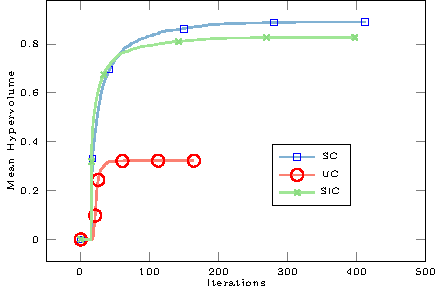
\includegraphics[width=0.3\textwidth]{CRA/SPEA2/charts/hypervolume/hv-mean-progression-b.pdf}}%
\hfill

\subcaptionbox{NSGA}{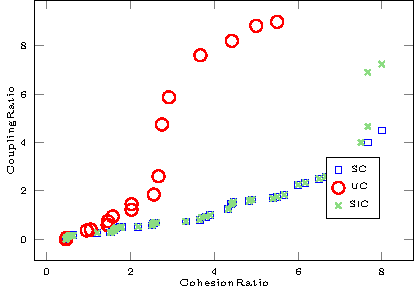
\includegraphics[width=0.3\textwidth]{CRA/NSGAII/charts/approximation_sets/approx-sets-B.pdf}}%
\hfill
\subcaptionbox{PESA2}{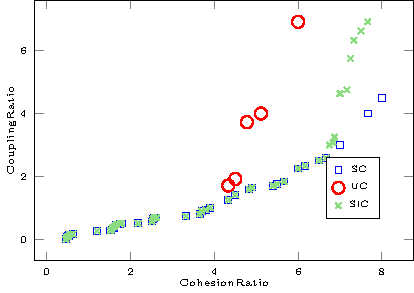
\includegraphics[width=0.3\textwidth]{CRA/PESA2/charts/approximation_sets/approx-sets-B.pdf}}%
\hfill
\subcaptionbox{SPEA2}{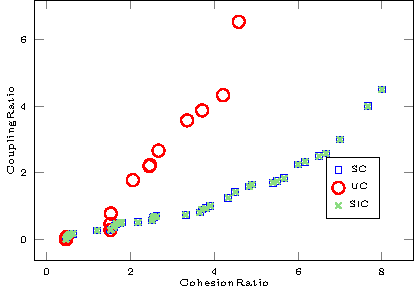
\includegraphics[width=0.3\textwidth]{CRA/SPEA2/charts/approximation_sets/approx-sets-B.pdf}}%
\hfill
\caption{Model B.}
\end{figure}

\clearpage

CRA case - Model C

\begin{figure}[h!]
\centering
\subcaptionbox{NSGA}{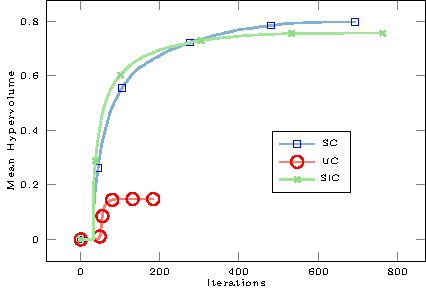
\includegraphics[width=0.3\textwidth]{CRA/NSGAII/charts/hypervolume/hv-mean-progression-c.pdf}}%
\hfill
\subcaptionbox{PESA2}{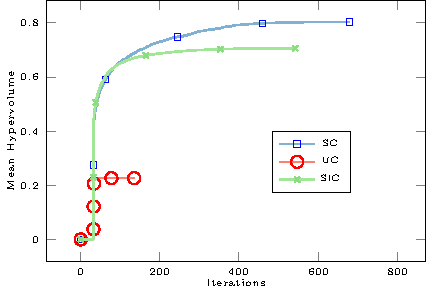
\includegraphics[width=0.3\textwidth]{CRA/PESA2/charts/hypervolume/hv-mean-progression-c.pdf}}%
\hfill
\subcaptionbox{SPEA2}{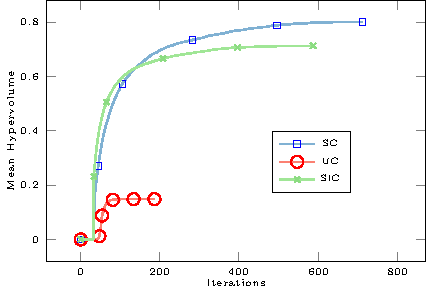
\includegraphics[width=0.3\textwidth]{CRA/SPEA2/charts/hypervolume/hv-mean-progression-c.pdf}}%
\hfill

\subcaptionbox{NSGA}{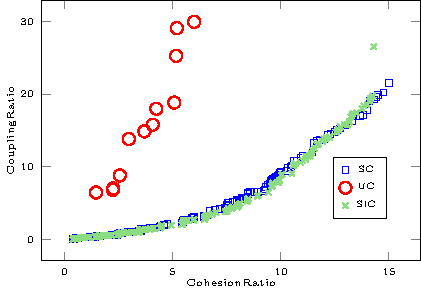
\includegraphics[width=0.3\textwidth]{CRA/NSGAII/charts/approximation_sets/approx-sets-C.pdf}}%
\hfill
\subcaptionbox{PESA2}{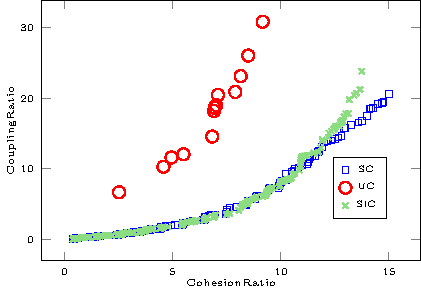
\includegraphics[width=0.3\textwidth]{CRA/PESA2/charts/approximation_sets/approx-sets-C.pdf}}%
\hfill
\subcaptionbox{SPEA2}{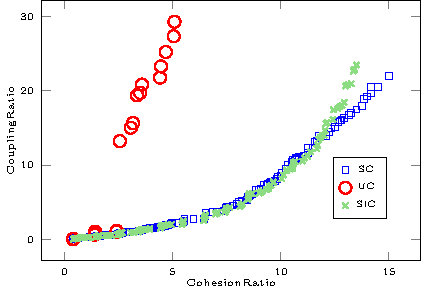
\includegraphics[width=0.3\textwidth]{CRA/SPEA2/charts/approximation_sets/approx-sets-C.pdf}}%
\hfill
\caption{Model C.}
\end{figure}

CRA case - Model D

\begin{figure}[h!]
\centering
\subcaptionbox{NSGA}{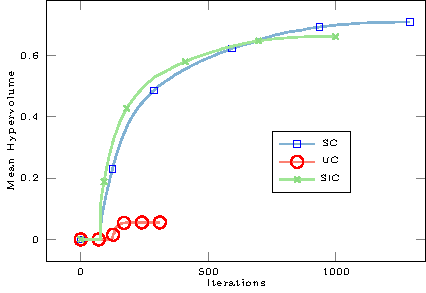
\includegraphics[width=0.3\textwidth]{CRA/NSGAII/charts/hypervolume/hv-mean-progression-d.pdf}}%
\hfill
\subcaptionbox{PESA2}{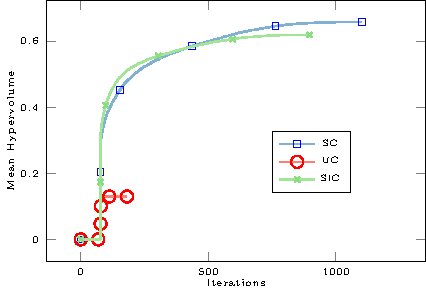
\includegraphics[width=0.3\textwidth]{CRA/PESA2/charts/hypervolume/hv-mean-progression-d.pdf}}%
\hfill
\subcaptionbox{SPEA2}{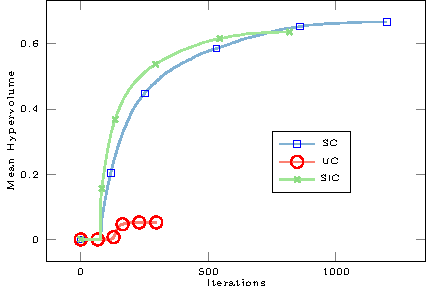
\includegraphics[width=0.3\textwidth]{CRA/SPEA2/charts/hypervolume/hv-mean-progression-d.pdf}}%
\hfill

\subcaptionbox{NSGA}{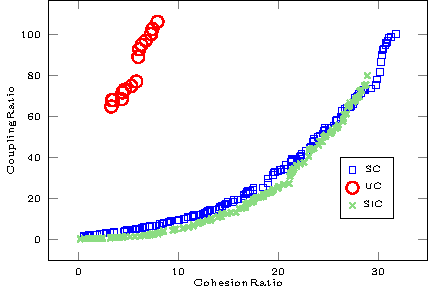
\includegraphics[width=0.3\textwidth]{CRA/NSGAII/charts/approximation_sets/approx-sets-D.pdf}}%
\hfill
\subcaptionbox{PESA2}{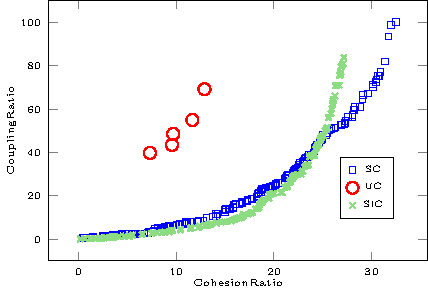
\includegraphics[width=0.3\textwidth]{CRA/PESA2/charts/approximation_sets/approx-sets-D.pdf}}%
\hfill
\subcaptionbox{SPEA2}{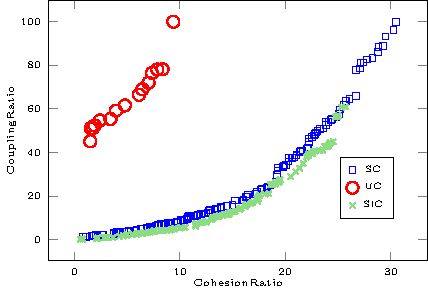
\includegraphics[width=0.3\textwidth]{CRA/SPEA2/charts/approximation_sets/approx-sets-D.pdf}}%
\hfill
\caption{Model D.}
\end{figure}

\clearpage

CRA case - Model E

\begin{figure}[h!]
\centering
\subcaptionbox{NSGA}{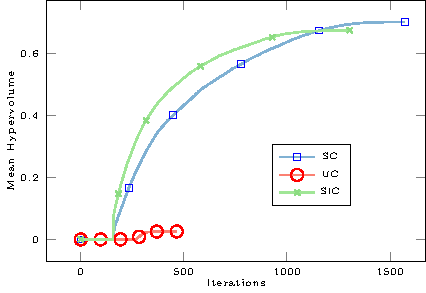
\includegraphics[width=0.3\textwidth]{CRA/NSGAII/charts/hypervolume/hv-mean-progression-e.pdf}}%
\hfill
\subcaptionbox{PESA2}{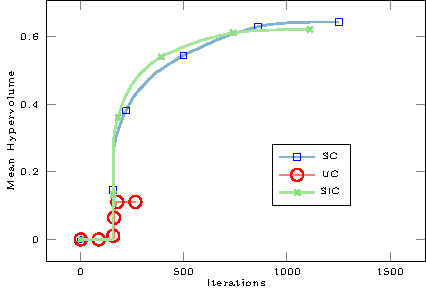
\includegraphics[width=0.3\textwidth]{CRA/PESA2/charts/hypervolume/hv-mean-progression-e.pdf}}%
\hfill
\subcaptionbox{SPEA2}{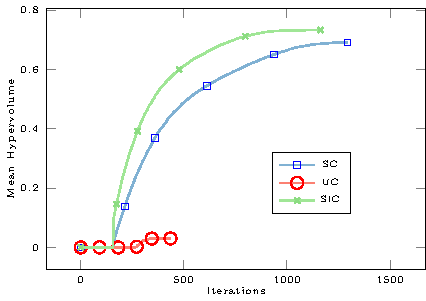
\includegraphics[width=0.3\textwidth]{CRA/SPEA2/charts/hypervolume/hv-mean-progression-e.pdf}}%
\hfill

\subcaptionbox{NSGA}{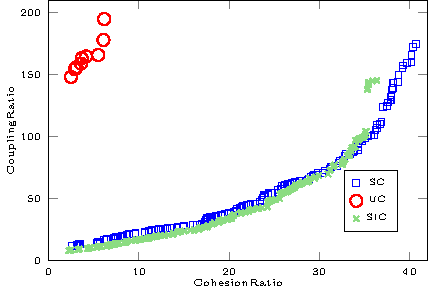
\includegraphics[width=0.3\textwidth]{CRA/NSGAII/charts/approximation_sets/approx-sets-E.pdf}}%
\hfill
\subcaptionbox{PESA2}{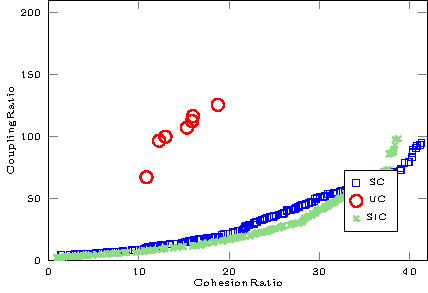
\includegraphics[width=0.3\textwidth]{CRA/PESA2/charts/approximation_sets/approx-sets-E.pdf}}%
\hfill
\subcaptionbox{SPEA2}{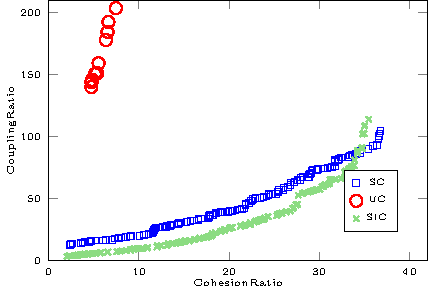
\includegraphics[width=0.3\textwidth]{CRA/SPEA2/charts/approximation_sets/approx-sets-E.pdf}}%
\hfill
\caption{Model E.}
\end{figure}

\clearpage

NRP case - Model A

\begin{figure}[h!]
\centering
\subcaptionbox{NSGA}{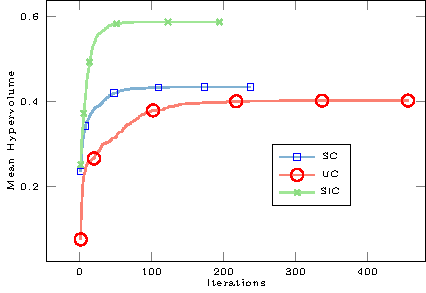
\includegraphics[width=0.3\textwidth]{NRP/NSGAII/charts/hypervolume/hv-mean-progression-a.pdf}}%
\hfill
\subcaptionbox{PESA2}{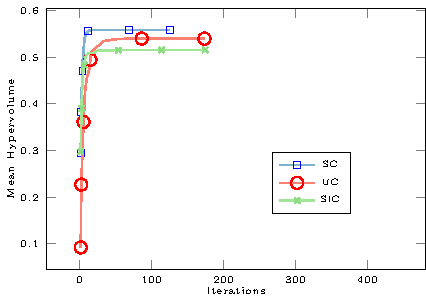
\includegraphics[width=0.3\textwidth]{NRP/PESA2/charts/hypervolume/hv-mean-progression-a.pdf}}%
\hfill
\subcaptionbox{SPEA2}{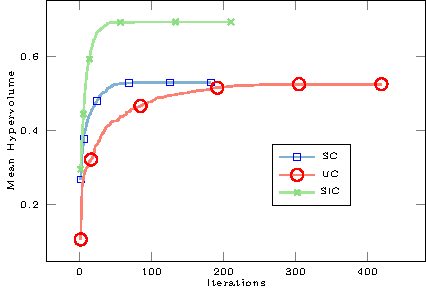
\includegraphics[width=0.3\textwidth]{NRP/SPEA2/charts/hypervolume/hv-mean-progression-a.pdf}}%
\hfill

\subcaptionbox{NSGA}{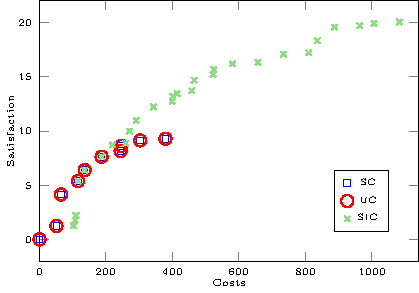
\includegraphics[width=0.3\textwidth]{NRP/NSGAII/charts/approximation_sets/approx-sets-A.pdf}}%
\hfill
\subcaptionbox{PESA2}{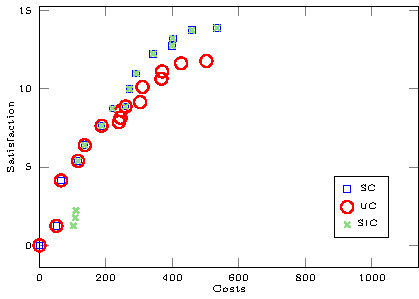
\includegraphics[width=0.3\textwidth]{NRP/PESA2/charts/approximation_sets/approx-sets-A.pdf}}%
\hfill
\subcaptionbox{SPEA2}{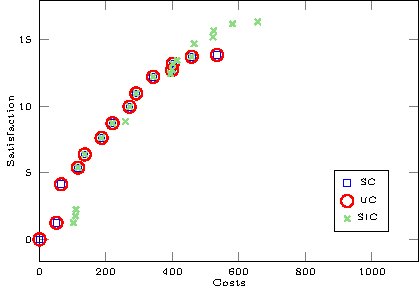
\includegraphics[width=0.3\textwidth]{NRP/SPEA2/charts/approximation_sets/approx-sets-A.pdf}}%
\hfill
\caption{Model A.}
\end{figure}

NRP case - Model B

\begin{figure}[h!]
\centering
\subcaptionbox{NSGA}{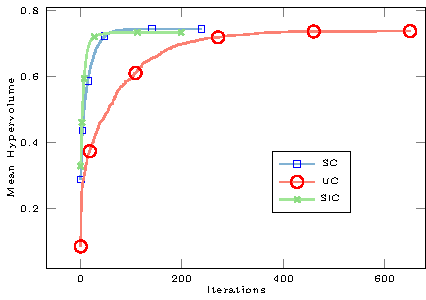
\includegraphics[width=0.3\textwidth]{NRP/NSGAII/charts/hypervolume/hv-mean-progression-b.pdf}}%
\hfill
\subcaptionbox{PESA2}{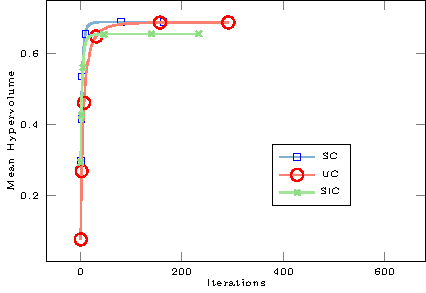
\includegraphics[width=0.3\textwidth]{NRP/PESA2/charts/hypervolume/hv-mean-progression-b.pdf}}%
\hfill
\subcaptionbox{SPEA2}{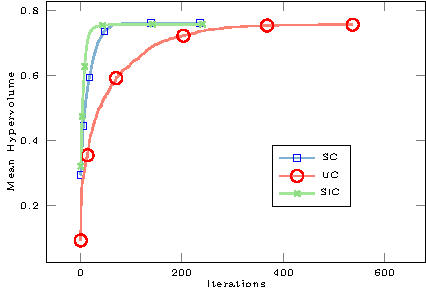
\includegraphics[width=0.3\textwidth]{NRP/SPEA2/charts/hypervolume/hv-mean-progression-b.pdf}}%
\hfill

\subcaptionbox{NSGA}{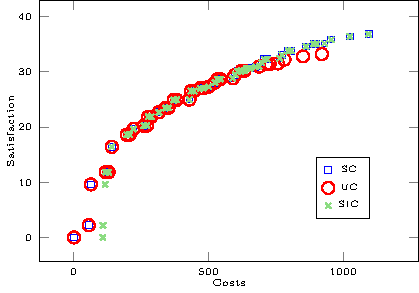
\includegraphics[width=0.3\textwidth]{NRP/NSGAII/charts/approximation_sets/approx-sets-B.pdf}}%
\hfill
\subcaptionbox{PESA2}{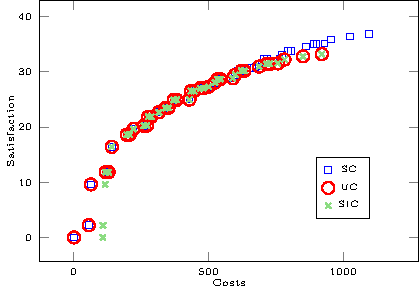
\includegraphics[width=0.3\textwidth]{NRP/PESA2/charts/approximation_sets/approx-sets-B.pdf}}%
\hfill
\subcaptionbox{SPEA2}{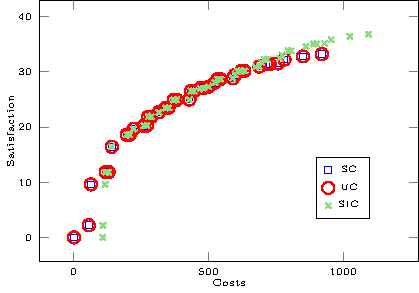
\includegraphics[width=0.3\textwidth]{NRP/SPEA2/charts/approximation_sets/approx-sets-B.pdf}}%
\hfill
\caption{Model B.}
\end{figure}

\clearpage

NRP case - Model C

\begin{figure}[h!]
\centering
\subcaptionbox{NSGA}{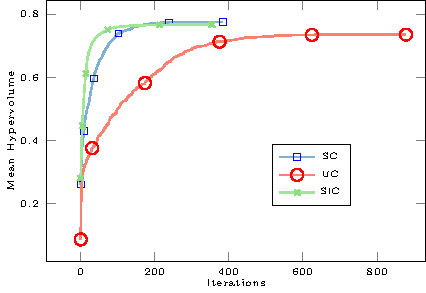
\includegraphics[width=0.3\textwidth]{NRP/NSGAII/charts/hypervolume/hv-mean-progression-c.pdf}}%
\hfill
\subcaptionbox{PESA2}{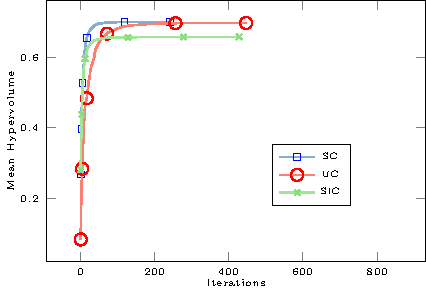
\includegraphics[width=0.3\textwidth]{NRP/PESA2/charts/hypervolume/hv-mean-progression-c.pdf}}%
\hfill
\subcaptionbox{SPEA2}{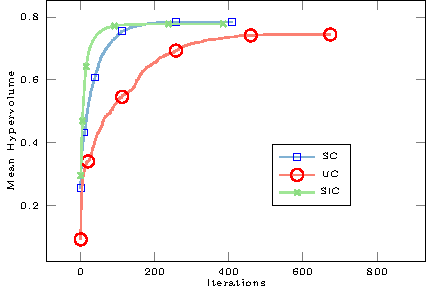
\includegraphics[width=0.3\textwidth]{NRP/SPEA2/charts/hypervolume/hv-mean-progression-c.pdf}}%
\hfill

\subcaptionbox{NSGA}{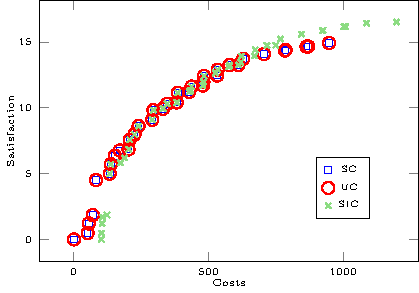
\includegraphics[width=0.3\textwidth]{NRP/NSGAII/charts/approximation_sets/approx-sets-C.pdf}}%
\hfill
\subcaptionbox{PESA2}{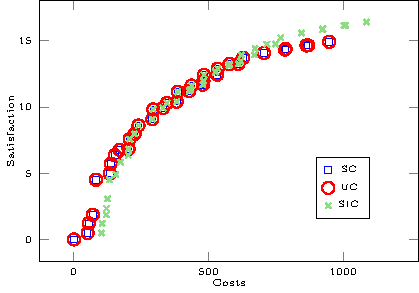
\includegraphics[width=0.3\textwidth]{NRP/PESA2/charts/approximation_sets/approx-sets-C.pdf}}%
\hfill
\subcaptionbox{SPEA2}{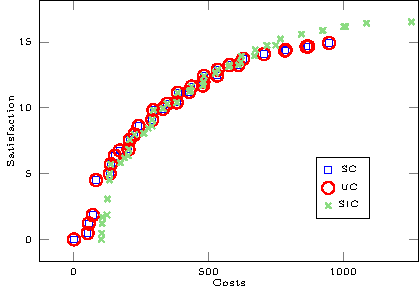
\includegraphics[width=0.3\textwidth]{NRP/SPEA2/charts/approximation_sets/approx-sets-C.pdf}}%
\hfill
\caption{Model C.}
\end{figure}


\clearpage

SCRUM case - Model A

\begin{figure}[h!]
\centering
\subcaptionbox{NSGA}{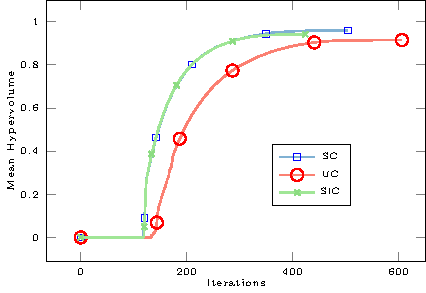
\includegraphics[width=0.3\textwidth]{SCRUM/NSGAII/charts/hypervolume/hv-mean-progression-a.pdf}}%
\hfill
\subcaptionbox{PESA2}{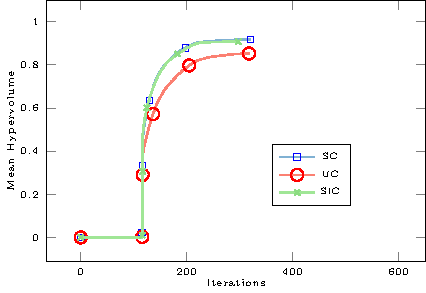
\includegraphics[width=0.3\textwidth]{SCRUM/PESA2/charts/hypervolume/hv-mean-progression-a.pdf}}%
\hfill
\subcaptionbox{SPEA2}{\includegraphics[width=0.3\textwidth]{SCRUM/SPEA2/charts/hypervolume/hv-mean-progression-a.pdf}}%
\hfill

\subcaptionbox{NSGA}{\includegraphics[width=0.3\textwidth]{SCRUM/NSGAII/charts/approximation_sets/approx-sets-A.pdf}}%
\hfill
\subcaptionbox{PESA2}{\includegraphics[width=0.3\textwidth]{SCRUM/PESA2/charts/approximation_sets/approx-sets-A.pdf}}%
\hfill
\subcaptionbox{SPEA2}{\includegraphics[width=0.3\textwidth]{SCRUM/SPEA2/charts/approximation_sets/approx-sets-A.pdf}}%
\hfill
\caption{Model A.}
\end{figure}

SCRUM case - Model B

\begin{figure}[h!]
\centering
\subcaptionbox{NSGA}{\includegraphics[width=0.3\textwidth]{SCRUM/NSGAII/charts/hypervolume/hv-mean-progression-b.pdf}}%
\hfill
\subcaptionbox{PESA2}{\includegraphics[width=0.3\textwidth]{SCRUM/PESA2/charts/hypervolume/hv-mean-progression-b.pdf}}%
\hfill
\subcaptionbox{SPEA2}{\includegraphics[width=0.3\textwidth]{SCRUM/SPEA2/charts/hypervolume/hv-mean-progression-b.pdf}}%
\hfill

\subcaptionbox{NSGA}{\includegraphics[width=0.3\textwidth]{SCRUM/NSGAII/charts/approximation_sets/approx-sets-B.pdf}}%
\hfill
\subcaptionbox{PESA2}{\includegraphics[width=0.3\textwidth]{SCRUM/PESA2/charts/approximation_sets/approx-sets-B.pdf}}%
\hfill
\subcaptionbox{SPEA2}{\includegraphics[width=0.3\textwidth]{SCRUM/SPEA2/charts/approximation_sets/approx-sets-B.pdf}}%
\hfill
\caption{Model B.}
\end{figure}


\clearpage

Takeaways:
\begin{itemize}
	\item Applying PESA2 UC is closer to SC and SIC in the CRA and SCRUM cases, however, it is still notably worse than the other sets.
	In the NRP case, however, SIC is less effective. Thereby, SIC becomes worse than SC and even worse than UC which gets very close to SC. 
	\item With UC PESA2 is not able to find the extremum where CouplingRatio is 0 in model A of CRA case.
	\item The performance of NSGA-II and SPEA2 is very similar with one exception: for the largest CRA model SIC outperforms SC.
	This could be a trend for larger models in general as there SIC comes closer to SC already for model D.
	
	
\end{itemize}


\end{document}